\chapter{المطيافية الإلكترونية والفيزياء الضوئية}\label{ch:b3:electronic-spectroscopy}

تحت مصباح الأشعة فوق البنفسجية في حانة معتمة، يتوهج كأس من المياه الفوارة المنكّهة بالكينين بزرقة
شاحبة شبحية. فالكينين الذي فيه يمتص الأشعة فوق البنفسجية، التي
لا تراها العين، ويعيد جزءًا منها بعد بضع نانوثوان ضوءًا
أزرق مرئيًا. امتصاص، فحياة قصيرة في حالة مثارة، فإصدار عند
طول موجة أطول، والطاقة التي لا تعود ضوءًا: فمصير
الجزيء المثار تنافس بين عمليات لها ثوابت سرعة،
وطيفه يتشكل باهتزازات الجزيء وبقواعد
التناظر في \cref{ch:b3:group-theory-applied}. يدرس هذا الفصل
الانتقالات الإلكترونية وما يحدث بعدها، وهو الموضوع المسمى
الفيزياء الضوئية؛ ويضيف \cref{ch:b3:photochemistry} الحالات التي يتفاعل فيها الجزيء
المثار.

\begin{recall}
قاس مجلد السنة الأولى الامتصاصية بقانون بير--لامبرت، $A =
\varepsilon\ell c$، وعرّف معامل الامتصاص المولي، وحوامل اللون
والأنظمة المترافقة، وربط اللون بقمة الامتصاص. وسمّى مجلد السنة الثانية
المدارات الحدودية HOMO وLUMO. وعرّف \cref{ch:b3:many-electron-atoms}
الحالتين الأحادية والثلاثية؛ و\cref{ch:b3:group-theory-applied} مبرهنة
التكاملات المعدومة؛ و\cref{ch:b3:rovibrational-spectroscopy}
المستويات الاهتزازية للرابطة.
\end{recall}

\begin{omfigure}
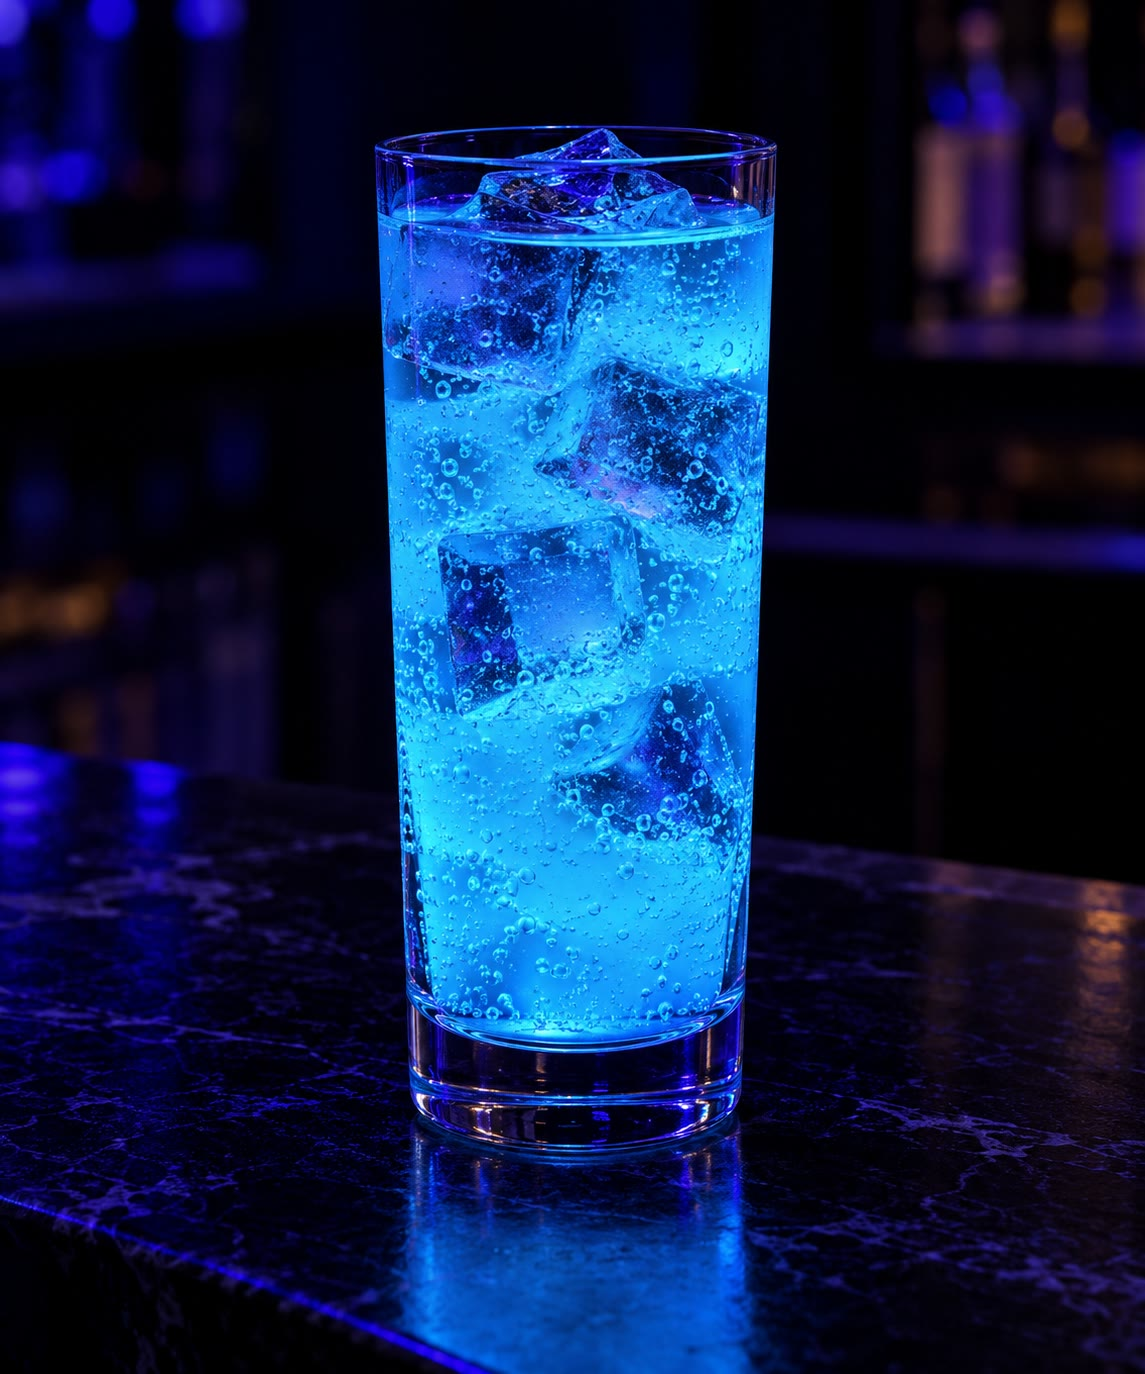
\includegraphics[height=4.6cm]{images/book4/ai/b3-07-tonic.jpg}\hspace{1em}%
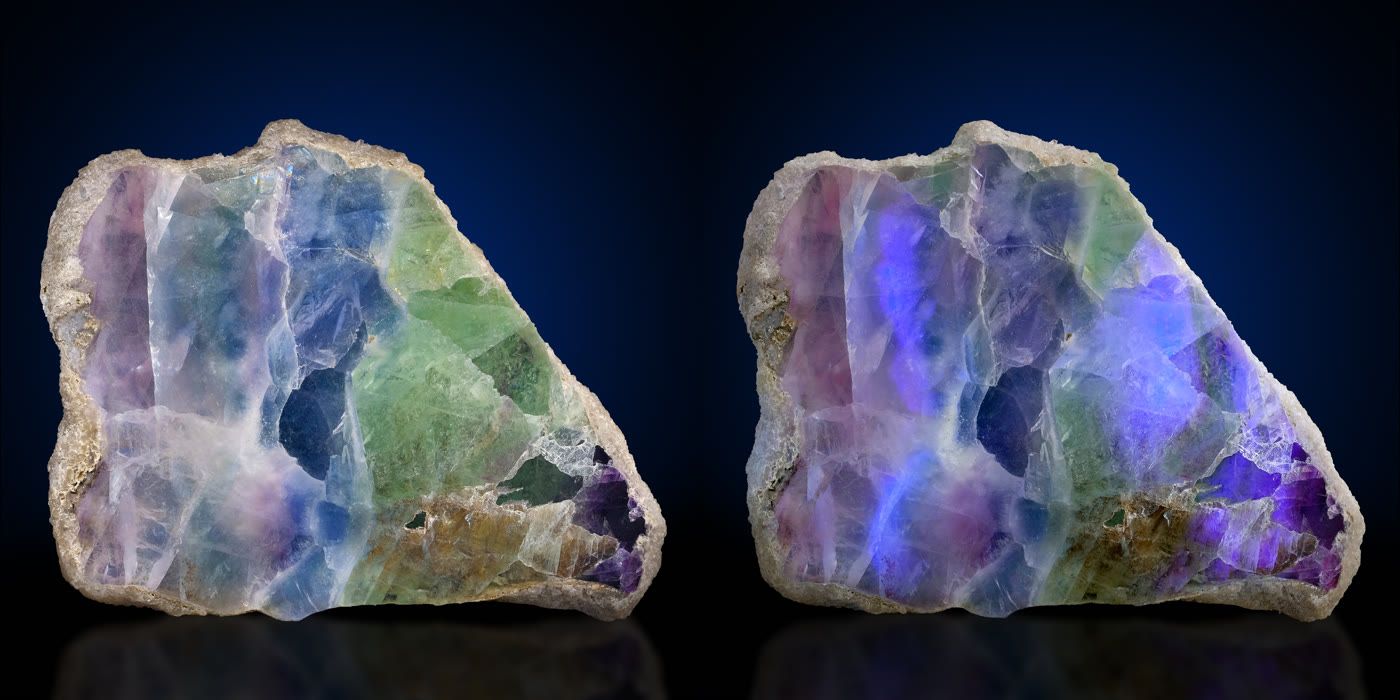
\includegraphics[height=4.6cm]{images/book4/fluorite-uv.jpg}

{\small يسارًا: مياه فوارة بالكينين تتوهج بالأزرق تحت مصباح للأشعة فوق البنفسجية. يمينًا:
الفلوريت في ضوء النهار ومتفلورًا تحت الأشعة فوق البنفسجية؛ وقد أعطى هذا المعدن
التفلورَ اسمه. الصورة: ماشا ميلشينا، CC BY 4.0.}
\end{omfigure}

\section{الانتقالات الإلكترونية وقواعد انتقائها}

\begin{definition}[عزم ثنائي القطب الانتقالي، قوة المذبذب]\label{def:b3:electronic-spectroscopy:transition-dipole}
\emph{عزم ثنائي القطب الانتقالي}\index{عزم ثنائي القطب الانتقالي} بين
الحالتين $\Psi_i$ و$\Psi_f$ هو $\boldsymbol\mu_{fi} = \langle\Psi_f|\hat{\boldsymbol\mu}|\Psi_i
\rangle$، حيث $\hat{\boldsymbol\mu} = -e\sum_k\mathbf r_k$ (مضافًا إليه شحنات
النوى، التي تُلغى بين حالتين متعامدتين). و\emph{قوة
المذبذب}\index{قوة المذبذب} $f$ هي المقياس اللابُعدي
لشدة حزمة، ونحو 1 لأشد الانتقالات.
\end{definition}

\begin{proposition}[الشدة وقوة المذبذب]\label{prop:b3:electronic-spectroscopy:intensity}
الامتصاص المكامَل لحزمة متناسب مع $|\boldsymbol\mu_{fi}|^2$،
وفي الممارسة
\[
f \approx 4.32\times10^{-9}\int\varepsilon(\tilde\nu)\,\dd\tilde\nu,
\]
حيث $\varepsilon$ بوحدة \unit{L.mol^{-1}.cm^{-1}} و$\tilde\nu$ بوحدة \unit{cm^{-1}}.
\end{proposition}
\admitted

يأتي التناسب من نظرية الاضطراب المتعلقة بالزمن، 
والعامل العددي من المذبذب الكلاسيكي؛ وكلاهما يُتناول في مقررات
أكثر تقدمًا. والمهم هنا أن $f$ لا تكون كبيرة إلا حين يكون
$\boldsymbol\mu_{fi}$ كبيرًا، وأن التناظر قد يفرض انعدامه.

\begin{theorem}[قاعدة الانتقاء السبينية]\label{thm:b3:electronic-spectroscopy:spin-rule}
الانتقال ثنائي القطب الكهربائي بين حالتين مختلفتي السبين الكلي
ممنوع: $\Delta S = 0$.
\end{theorem}

\begin{proof}
كل حالة جداء دالة فضائية ودالة سبين، $\Psi = \phi\,\chi$.
\omterm{def:b3:quantum-model-systems:operator}{ومؤثر} ثنائي القطب لا يؤثر إلا في المواضع، فيكون $\langle\phi_f\chi_f|\hat{\boldsymbol\mu}|
\phi_i\chi_i\rangle = \langle\phi_f|\hat{\boldsymbol\mu}|\phi_i\rangle\langle\chi_f|\chi_i\rangle$.
ودوال السبين ذات قيم $S$ المختلفة دوال ذاتية \omterm{def:b3:quantum-model-systems:operator}{للمؤثر} $\hat S^2$ بقيم ذاتية
مختلفة، فهي متعامدة (\cref{thm:b3:quantum-model-systems:hermitian-real}):
فينعدم العامل الثاني.
\end{proof}

\begin{theorem}[قاعدة لابورت]\label{thm:b3:electronic-spectroscopy:laporte}
في جزيء له \omterm{def:b3:point-groups:inversion}{مركز انقلاب}، يجب أن يغيّر الانتقال ثنائي القطب الكهربائي
الزوجية: فالانتقال $g \leftrightarrow u$ مسموح، و$g \leftrightarrow g$ و$u
\leftrightarrow u$ ممنوعان. هذه هي \emph{قاعدة لابورت}\index{قاعدة لابورت}.
\end{theorem}

\begin{proof}
مركبات $\hat{\boldsymbol\mu}$ تغيّر إشارتها تحت الانقلاب: فهي $u$.
والجداء $\Gamma_f\otimes\Gamma_\mu\otimes\Gamma_i$ لا يكون $g$ إلا إذا كان للتمثيلين $\Gamma_f$ و$\Gamma_i$
زوجيتان متعاكستان؛ وإلا كان $u$ ولم يمكن أن يحتوي \omterm{def:b3:group-theory-applied:reducible}{التمثيل المتناظر
كليًا} (\cref{thm:b3:group-theory-applied:vanishing-integral}).
\end{proof}

القاعدتان صارمتان في الحالات المثالية؛ أما الجزيئات الحقيقية فتخففهما
--- \omterm{def:b3:many-electron-atoms:spin-orbit}{فاقتران السبين--المدار} يمزج الطابعين الأحادي والثلاثي، والاهتزازات
تزيل مركز التناظر لحظةً --- فتظهر الانتقالات «الممنوعة»،
ضعيفة. وحزم \babelsublr{$d$--$d$} في المعقدات الثمانية الأوجه، الممنوعة \omterm{thm:b3:electronic-spectroscopy:laporte}{بقاعدة لابورت}
والضعيفة، تدين بلونها لهذا التخفيف
(\cref{ch:b3:complex-spectra-magnetism}).

\begin{definition}[انتقال نقل الشحنة]\label{def:b3:electronic-spectroscopy:charge-transfer}
\emph{انتقال نقل الشحنة}\index{انتقال نقل الشحنة} ينقل
إلكترونًا من مدار متمركز أساسًا على جزء من نظام (مانح) إلى
مدار متمركز أساسًا على جزء آخر (مستقبل)؛ \omterm{def:b3:electronic-spectroscopy:transition-dipole}{وعزم ثنائي القطب الانتقالي} فيه
كبير، وحزمته شديدة وعريضة، وطاقته حساسة لقطبية
المذيب.
\end{definition}

\begin{method}[إسناد حزمة امتصاص]\label{met:b3:electronic-spectroscopy:assign-band}
\begin{enumerate}
  \item $\varepsilon_{\max}$ فوق نحو \qty{e4}{L.mol^{-1}.cm^{-1}}: انتقال
        مسموح ($\pi\to\pi^*$ في نظام مترافق، أو نقل شحنة).
  \item $\varepsilon_{\max}$ من 10 إلى بضع مئات: انتقال ممنوع ($n\to\pi^*$،
        ممنوع بالتناظر؛ \babelsublr{$d$--$d$}، ممنوع \omterm{thm:b3:electronic-spectroscopy:laporte}{بقاعدة لابورت}).
  \item $\varepsilon_{\max}$ دون 1: ممنوع سبينيًا.
  \item تنزاح حزمة $n\to\pi^*$ نحو أطوال موجية أقصر في المذيبات البروتونية
        (فالزوج الحر يستقر بالروابط الهيدروجينية)، وتنزاح حزمة $\pi\to\pi^*$
        عادة نحو أطوال أطول.
\end{enumerate}
\end{method}

\section{مبدأ فرانك--كوندون}

\begin{theorem}[مبدأ فرانك--كوندون]\label{thm:b3:electronic-spectroscopy:franck-condon}
في إطار \omterm{def:b3:computational-chemistry:born-oppenheimer}{تقريب بورن--أوبنهايمر}، وإذا كان \omterm{def:b3:electronic-spectroscopy:transition-dipole}{عزم ثنائي القطب الانتقالي}
قليل التعلق بمواضع النوى، فإن شدة \omterm{def:b3:electronic-spectroscopy:vibronic}{الانتقال الاهتزازي الإلكتروني}
من المستوى الاهتزازي $v''$ للحالة الإلكترونية الدنيا إلى المستوى
$v'$ للحالة العليا متناسبة مع $|\langle\chi_{v'}|\chi_{v''}\rangle|^2$، أي
مربع تداخل الدالتين الموجيتين الاهتزازيتين: هذا هو
\emph{مبدأ فرانك--كوندون}\index{مبدأ فرانك--كوندون}. فالانتقالات
الإلكترونية عمودية: النوى لا تتحرك بينما تقفز الإلكترونات.
\end{theorem}

\begin{proof}
مع $\Psi = \psi_{\mathrm{el}}(\mathbf r;R)\chi_v(R)$، يكون عزم الانتقال
$\int\chi_{v'}^*\big[\int\psi'^*_{\mathrm{el}}\hat\mu\psi''_{\mathrm{el}}\dd\mathbf r\big]
\chi_{v''}\,\dd R$. وما بين المعقوفين هو عزم الانتقال الإلكتروني
$\mu_{\mathrm{el}}(R)$؛ وإذا أُخذ ثابتًا (تقريب كوندون)، خرج من
التكامل، فيبقى $\mu_{\mathrm{el}}\langle\chi_{v'}|\chi_{v''}\rangle$.
\end{proof}

\begin{definition}[الانتقال الاهتزازي الإلكتروني، المتوالية، عامل فرانك--كوندون]\label{def:b3:electronic-spectroscopy:vibronic}
\emph{الانتقال الاهتزازي الإلكتروني}\index{انتقال اهتزازي إلكتروني} يغيّر الحالتين الإلكترونية
والاهتزازية معًا؛ والخطوط $v' \leftarrow 0$ من أجل $v' = 0, 1, 2,
\dots$ تشكّل \emph{متوالية اهتزازية إلكترونية}\index{متوالية اهتزازية إلكترونية}؛ 
و\emph{عامل فرانك--كوندون}\index{عامل فرانك--كوندون} لخط اهتزازي إلكتروني هو
$|\langle\chi_{v'}|\chi_{v''}\rangle|^2$.
\end{definition}

\begin{proposition}[المذبذبات المزاحة]\label{prop:b3:electronic-spectroscopy:displaced}
إذا كانت الحالتان توافقيتين بالتردد نفسه وكانت قيمة الحالة العليا الدنيا
مزاحة بمقدار $\Delta$ (بوحدات $\sqrt{\hbar/m\omega}$)، فإن عوامل فرانك--كوندون
انطلاقًا من $v'' = 0$ تشكّل توزيع بواسون،
$|\langle v'|0\rangle|^2 = \eu^{-S}S^{v'}/v'!$، حيث $S = \Delta^2/2$؛ والخط الأشد
قرب $v' = S$.
\end{proposition}
\admitted

يستعمل البرهان العام \omterm{def:b3:quantum-model-systems:ladder}{مؤثرات السلّم} في
\cref{ch:b3:quantum-model-systems}؛ وتتحقق معطيات أشكال هذا الفصل من
العلاقة بالمكاملة المباشرة. فالإزاحة الصغيرة تعطي خطًا قويًا واحدًا
0--0؛ والإزاحة الكبيرة متواليةً طويلة يقع أشد أعضائها بعيدًا عن
الخط 0--0.

\begin{omfigure}
\begin{tikzpicture}
\begin{axis}[name=pc, width=0.46\linewidth, height=6cm, xmin=-4, xmax=5, ymin=0,
  ymax=14, axis lines=left, xtick=\empty, ytick=\empty, xlabel={\foreignlanguage{arabic}{الإحداثي النووي}},
  ylabel={\foreignlanguage{arabic}{الطاقة}}, label style={font=\small}]
\addplot[black, thick] table[x=y, y=ground] {figdata/out/bachelor-3-franck-condon-curves.dat};
\addplot[omDef, thick] table[x=y, y=excited] {figdata/out/bachelor-3-franck-condon-curves.dat};
\draw[omabs] (axis cs:0,0.5) -- (axis cs:0,10.6);
\draw[omvib] (axis cs:-1,0.5) -- (axis cs:1,0.5);
\draw[omvib] (axis cs:0.732,9.5) -- (axis cs:2.732,9.5);
\draw[omvib] (axis cs:-0.000,10.5) -- (axis cs:3.464,10.5);
\draw[omvib] (axis cs:-0.504,11.5) -- (axis cs:3.968,11.5);
\draw[omvib] (axis cs:-0.914,12.5) -- (axis cs:4.378,12.5);
\node[font=\small, anchor=west] at (axis cs:-3.9,13.0) {\foreignlanguage{arabic}{مثارة}};
\node[font=\small, anchor=west] at (axis cs:3.0,1.5) {\foreignlanguage{arabic}{أساسية}};
\node[font=\scriptsize, anchor=east] at (axis cs:-0.05,5.5) {\foreignlanguage{arabic}{انتقال عمودي}};
\end{axis}
\begin{axis}[at={(pc.east)}, anchor=west, xshift=1.3cm, width=0.46\linewidth,
  height=6cm, xmin=-0.5, xmax=12.5, ymin=0, ymax=0.8, axis lines=left, ycomb,
  xlabel={$v'$}, ylabel={\foreignlanguage{arabic}{عامل فرانك--كوندون}}, label style={font=\small},
  tick label style={font=\small}]
\addplot[black, very thick] table[x=v, y=s03] {figdata/out/bachelor-3-franck-condon-sticks.dat};
\addplot[omDef, very thick, xshift=2pt] table[x=v, y=s15] {figdata/out/bachelor-3-franck-condon-sticks.dat};
\addplot[omThm, very thick, xshift=4pt] table[x=v, y=s5] {figdata/out/bachelor-3-franck-condon-sticks.dat};
\end{axis}
\end{tikzpicture}

{\small يسارًا: انتقال عمودي من أدنى مستوى للحالة الأساسية
يحطّ حيث يكون المنحنى المثار، المزاح نحو طول رابطة أكبر، عاليًا فوق
قاعه (مرسوم من أجل $S = 1.5$). يمينًا: عوامل فرانك--كوندون في
المتوالية من أجل $S = 0.3$ (أسود) و1.5 (أزرق) و5 (أحمر)؛ ومجموع كل مجموعة
يساوي 1.}
\end{omfigure}

\begin{example}[اليود]\label{ex:b3:electronic-spectroscopy:iodine}
% ledger: diat:I2.re, diat:I2B.re, diat:I2B.we, imass:I127
بخار اليود بنفسجي لأن حزمته \babelsublr{B$\leftarrow$X} تمتص الضوء الأصفر المخضر.
وتطول الرابطة من \qty{266.6}{pm} في الحالة الأساسية إلى \qty{302.5}{pm} في
الحالة B. وفي نموذج المذبذبات المزاحة بتردد الحالة B
(\qty{125.7}{cm^{-1}})، يعطي $\Delta R = \qty{35.8}{pm}$ القيمة $S \approx 15$: فالامتصاص
متوالية طويلة تنتهي أشد خطوطها على مستويات اهتزازية عالية للحالة
B، ويمتد آخرها في متصل التفكك.
\end{example}

\section{مصائر الحالة المثارة: مخطط يابلونسكي}

\begin{definition}[مخطط يابلونسكي]\label{def:b3:electronic-spectroscopy:jablonski}
\emph{مخطط يابلونسكي}\index{مخطط يابلونسكي} يبيّن الحالات الإلكترونية
لجزيء (الحالات الأحادية $S_0, S_1, S_2, \dots$ في عمود، والثلاثية $T_1, T_2,
\dots$ في آخر)، ومستوياتها الاهتزازية، والعمليات التي تصل بينها:
الإشعاعية بأسهم مستقيمة، واللاإشعاعية بأسهم متموجة.
\end{definition}

\begin{definition}[العمليات اللاإشعاعية]\label{def:b3:electronic-spectroscopy:radiationless}
يُنزل \emph{الاسترخاء الاهتزازي}\index{استرخاء اهتزازي} الجزيءَ المثار
إلى أدنى مستوى اهتزازي في حالته الإلكترونية بالتصادمات،
في بضع بيكوثوان. و\emph{التحول الداخلي}\index{تحول داخلي}
انتقال لاإشعاعي بين حالتين لهما
التعددية نفسها ($S_2 \to S_1$، $S_1 \to S_0$)؛ و\emph{العبور بين
الأنظمة}\index{عبور بين الأنظمة} انتقال بين حالتين مختلفتي
التعددية ($S_1 \to T_1$، $T_1 \to S_0$).
\end{definition}

\begin{definition}[التألق، التفلور، التفسفر، انزياح ستوكس]\label{def:b3:electronic-spectroscopy:luminescence}
\emph{التألق}\index{تألق} إصدار جزيء مثار
للضوء. و\emph{التفلور}\index{تفلور} إصدار مسموح سبينيًا،
عادة $S_1 \to S_0$، سريع (نانوثوان)؛ و\emph{التفسفر}\index{تفسفر}
إصدار ممنوع سبينيًا، عادة $T_1 \to S_0$، بطيء (من الميلي ثانية إلى
الثواني). و\emph{انزياح ستوكس}\index{انزياح ستوكس} هو الفرق بين
قمتي الامتصاص والإصدار، مقدَّرًا بالطاقة.
\end{definition}

\begin{omfigure}
\begin{tikzpicture}[font=\small, >=Stealth]
  \foreach \y/\l in {0/{$S_0$}, 3.4/{$S_1$}, 5.6/{$S_2$}}{
    \draw[omstate] (0,\y) -- (3.6,\y); \node[anchor=east] at (-0.1,\y) {\l};
    \foreach \d in {0.25,0.5,0.75}{\draw[omvib] (0,\y+\d) -- (3.6,\y+\d);}}
  \draw[omstate] (5.0,2.5) -- (7.6,2.5); \node[anchor=west] at (7.7,2.5) {$T_1$};
  \foreach \d in {0.25,0.5,0.75}{\draw[omvib] (5.0,2.5+\d) -- (7.6,2.5+\d);}
  \draw[omabs] (0.3,0) -- (0.3,4.15) node[pos=0.35, left, font=\scriptsize, align=right] {\foreignlanguage{arabic}{امتصاص}};
  \draw[omabs] (0.7,0) -- (0.7,5.85);
  \draw[omnonrad] (1.05,5.85) -- (1.05,5.6);
  \draw[omnonrad] (1.05,5.6) -- (1.05,3.4) node[pos=0.5, right, font=\scriptsize] {IC};
  \draw[omnonrad] (0.45,4.15) -- (0.45,3.42);
  \draw[omfluo] (1.7,3.4) -- (1.7,0.5) node[pos=0.5, right, font=\scriptsize, align=left] {\foreignlanguage{arabic}{تفلور}};
  \draw[omnonrad] (3.2,3.4) -- (3.2,0.02) node[pos=0.5, right, font=\scriptsize] {IC};
  \draw[omisc] (3.6,3.4) -- (5.0,3.1) node[pos=0.5, above, font=\scriptsize] {ISC};
  \draw[omnonrad] (5.3,3.1) -- (5.3,2.52);
  \draw[omphos] (6.0,2.5) -- (6.0,0.5) node[pos=0.5, right, font=\scriptsize, align=left] {\foreignlanguage{arabic}{تفسفر}};
  \draw[omisc] (5.6,2.5) -- (3.7,0.02) node[pos=0.45, above left, font=\scriptsize, inner sep=1pt] {ISC};
  \draw[omvib, dashed] (3.6,0.5) -- (6.0,0.5);
  \draw[omvib, dashed] (3.6,0.0) -- (7.6,0.0);
\end{tikzpicture}

{\small \omterm{def:b3:electronic-spectroscopy:jablonski}{مخطط يابلونسكي}. الأسهم المستقيمة: الامتصاص (أزرق)، \omterm{def:b3:electronic-spectroscopy:luminescence}{والتفلور}
(أحمر)، \omterm{def:b3:electronic-spectroscopy:luminescence}{والتفسفر} (برتقالي)؛ والأسهم المتموجة: \omterm{def:b3:electronic-spectroscopy:radiationless}{الاسترخاء الاهتزازي} 
\omterm{def:b3:electronic-spectroscopy:radiationless}{والتحول الداخلي} (IC)؛ والأسهم المتموجة المتقطعة: \omterm{def:b3:electronic-spectroscopy:radiationless}{العبور بين الأنظمة} (ISC).
يبدأ الإصدار من أدنى مستوى اهتزازي في $S_1$ أو $T_1$ ويمكن أن ينتهي
على أي مستوى من مستويات $S_0$.}
\end{omfigure}

\begin{proposition}[قاعدة كاشا]\label{prop:b3:electronic-spectroscopy:kasha}
يحدث \omterm{def:b3:electronic-spectroscopy:luminescence}{التألق}، باستثناءات قليلة جدًا، من أدنى حالة مثارة
ذات تعددية معينة ($S_1$ أو $T_1$)، أيًا كانت الحالة التي أُثيرت أولًا:
وهذه \emph{قاعدة كاشا}\index{قاعدة كاشا}.
\end{proposition}
\begin{proof}[مكانتها]
مثبتة تجريبيًا؛ وسببها أن \omterm{def:b3:electronic-spectroscopy:radiationless}{التحول الداخلي} بين
الحالات المثارة العليا، المتقاربة، أسرع بكثير من الإصدار،
بينما الفجوة \babelsublr{$S_1$--$S_0$} كبيرة.
\end{proof}

\begin{proposition}[الخيال المرآوي]\label{prop:b3:electronic-spectroscopy:mirror}
إذا كانت للحالتين المثارة والأساسية بنيتان اهتزازيتان متشابهتان، كانت
حزمة \omterm{def:b3:electronic-spectroscopy:luminescence}{التفلور} خيالًا مرآويًا لحزمة الامتصاص الأولى بالنسبة إلى خطهما
المشترك 0--0؛ ويقع الإصدار عند أطوال موجية أطول (\omterm{def:b3:electronic-spectroscopy:luminescence}{انزياح ستوكس}).
\end{proposition}

\begin{proof}
ينطلق الامتصاص من $v'' = 0$ إلى مستويات $v'$ للحالة $S_1$، عند $E_{00} + v'h\nu'$؛ وينطلق الإصدار
من $v' = 0$ إلى مستويات $v''$ للحالة $S_0$، عند $E_{00} - v''h\nu''$. ومع تساوي
الترددين وتساوي عوامل فرانك--كوندون (الإزاحة نفسها)، تكون
المتواليتان متناظرتين بالنسبة إلى $E_{00}$.
\end{proof}

\begin{omfigure}
\begin{tikzpicture}
\begin{axis}[width=0.75\linewidth, height=5cm, xmin=17, xmax=33, ymin=0,
  ymax=1.15, axis x line=bottom, axis y line=left, ytick=\empty,
  xlabel={\foreignlanguage{arabic}{العدد الموجي \babelsublr{($10^3$ cm$^{-1}$)}}}, ylabel={\foreignlanguage{arabic}{الشدة}},
  legend cell align=left, legend style={font=\small, draw=none, at={(0.02,0.97)}, anchor=north west},
  tick label style={font=\small}, label style={font=\small}]
\addplot[omDef, thick] table[x=nu, y=abs] {figdata/out/bachelor-3-photophysics-bands.dat};
\addlegendentry{\foreignlanguage{arabic}{امتصاص}}
\addplot[omThm, thick] table[x=nu, y=em] {figdata/out/bachelor-3-photophysics-bands.dat};
\addlegendentry{\foreignlanguage{arabic}{تفلور}}
\draw[gray, dashed] (axis cs:25,0) -- (axis cs:25,1.12);
\node[font=\scriptsize, gray, anchor=south west] at (axis cs:25,1.0) {0--0};
\end{axis}
\end{tikzpicture}

{\small امتصاص جزيء نموذجي وتفلوره ($S = 1$، والكمّ
الاهتزازي \qty{1400}{cm^{-1}}): خيالان مرآويان بالنسبة إلى الخط 0--0؛ ويفصل
بين قمتيهما \omterm{def:b3:electronic-spectroscopy:luminescence}{انزياح ستوكس}.}
\end{omfigure}

\section{حركية الحالات المثارة}

بعد الإثارة، يتناقص إشغال $S_1$ بكل عملية متاحة له،
وكل منها من الرتبة الأولى: التفكك الإشعاعي $k_r$، \omterm{def:b3:electronic-spectroscopy:radiationless}{والتحول الداخلي} $k_{\mathrm{IC}}$،
\omterm{def:b3:electronic-spectroscopy:radiationless}{والعبور بين الأنظمة} $k_{\mathrm{ISC}}$.

\begin{definition}[عمر الحالة المثارة، العمر الإشعاعي]\label{def:b3:electronic-spectroscopy:lifetime}
\emph{عمر الحالة المثارة}\index{عمر الحالة المثارة} هو $\tau =
1/\sum k$، ثابت الزمن للتناقص الأسي لإشغال الحالة
المثارة. و\emph{العمر الإشعاعي}\index{عمر إشعاعي} $\tau_r =
1/k_r$ هو العمر الذي كانت الحالة ستملكه لو كان الإصدار مصيرها
الوحيد.
\end{definition}

\begin{definition}[المردود الكمي]\label{def:b3:electronic-spectroscopy:quantum-yield}
\emph{المردود الكمي}\index{مردود كمي} لعملية تلي
امتصاص الضوء هو عدد أحداث تلك العملية مقسومًا على
عدد الفوتونات الممتصة. و\emph{المردود الكمي
للتفلور}\index{مردود كمي للتفلور} $\Phi_F$ هو عدد الفوتونات
المصدرة تفلورًا لكل فوتون ممتص.
\end{definition}

\begin{proposition}[المردود الكمي والعمر]\label{prop:b3:electronic-spectroscopy:quantum-yield}
$\Phi_F = k_r/(k_r + k_{\mathrm{IC}} + k_{\mathrm{ISC}}) = k_r\tau = \tau/\tau_r$؛ وبالمثل
$\Phi_{\mathrm{ISC}} = k_{\mathrm{ISC}}\tau$، ومجموع مردودات العمليات المتنافسة
يساوي 1.
\end{proposition}

\begin{proof}
$\dd[S_1]/\dd t = -(k_r + k_{\mathrm{IC}} + k_{\mathrm{ISC}})[S_1]$، ومنه $[S_1] = [S_1]_0\eu^{-t/\tau}$.
وعدد الفوتونات المصدرة هو $\int_0^\infty k_r[S_1]\,\dd t = k_r\tau[S_1]_0$، من أصل
$[S_1]_0$ جزيء مثار. والتكامل نفسه مع كل $k$ يعطي كل مردود،
ومجموعها $\tau\sum k = 1$.
\end{proof}

\begin{definition}[مخمد التفلور، الإخماد الديناميكي والسكوني]\label{def:b3:electronic-spectroscopy:quencher}
\emph{مخمد التفلور}\index{مخمد التفلور} نوع كيميائي
يُضعف \omterm{def:b3:electronic-spectroscopy:luminescence}{التفلور}. ففي \emph{الإخماد الديناميكي}\index{إخماد ديناميكي}
يعطّل المخمدُ الجزيءَ المثار عند التصادم، مضيفًا سرعة $k_q[Q]$ 
ومقصّرًا العمر؛ وفي \emph{الإخماد السكوني}\index{إخماد سكوني}
يكوّن مع الجزيء في الحالة الأساسية معقدًا غير متفلور، فيُنقص
الشدة دون تغيير عمر الجزيئات التي ما زالت تُصدر.
\end{definition}

\begin{theorem}[معادلة شتيرن--فولمر]\label{thm:b3:electronic-spectroscopy:stern-volmer}
من أجل \omterm{def:b3:electronic-spectroscopy:quencher}{الإخماد الديناميكي}،
\[
\frac{I_0}{I} = \frac{\tau_0}{\tau} = 1 + k_q\tau_0[Q] = 1 + K_{SV}[Q],
\]
وهي \emph{معادلة شتيرن--فولمر}\index{معادلة شتيرن--فولمر}، حيث $I_0$ و$\tau_0$
مقيستان دون مخمد و$K_{SV} = k_q\tau_0$.
\end{theorem}

\begin{proof}
بوجود المخمد، $\tau = 1/(k_0 + k_q[Q])$ حيث $k_0 = 1/\tau_0$، ومنه $\tau_0/\tau = 1 +
k_q\tau_0[Q]$. والشدة متناسبة مع $\Phi_F = k_r\tau$، ومنه $I_0/I = \tau_0/\tau$.
\end{proof}

\begin{omfigure}
\begin{tikzpicture}
\begin{axis}[name=dec, width=0.5\linewidth, height=5cm, xmin=0, xmax=40, ymode=log,
  ymin=0.005, ymax=1.2, axis lines=left, xlabel={\babelsublr{$t$ / ns}}, ylabel={$I(t)/I(0)$},
  legend cell align=left, legend style={font=\scriptsize, draw=none, at={(0.98,0.98)}, anchor=north east},
  tick label style={font=\small}, label style={font=\small}]
\addplot[black, thick] table[x=t, y=q0] {figdata/out/bachelor-3-photophysics-decays.dat};
\addlegendentry{$[Q] = 0$}
\addplot[omDef, thick] table[x=t, y=q1] {figdata/out/bachelor-3-photophysics-decays.dat};
\addlegendentry{\babelsublr{0.01 M}}
\addplot[omProp, thick] table[x=t, y=q2] {figdata/out/bachelor-3-photophysics-decays.dat};
\addlegendentry{\babelsublr{0.02 M}}
\addplot[omThm, thick] table[x=t, y=q4] {figdata/out/bachelor-3-photophysics-decays.dat};
\addlegendentry{\babelsublr{0.04 M}}
\end{axis}
\begin{axis}[at={(dec.east)}, anchor=west, xshift=1.4cm, width=0.42\linewidth,
  height=5cm, xmin=0, xmax=0.045, ymin=0, ymax=3.3, axis lines=left,
  xlabel={\babelsublr{$[Q]$ / mol L$^{-1}$}}, ylabel={$I_0/I = \tau_0/\tau$},
  xticklabel style={/pgf/number format/fixed, /pgf/number format/precision=2},
  scaled x ticks=false, tick label style={font=\small}, label style={font=\small}]
\addplot[omThm, thick, mark=*] table[x=Q, y=I0I] {figdata/out/bachelor-3-photophysics-sv.dat};
\end{axis}
\end{tikzpicture}

{\small \omterm{def:b3:electronic-spectroscopy:quencher}{الإخماد الديناميكي} لمتفلور نموذجي ($\tau_0 = \qty{10}{ns}$، $k_q =
\qty{5e9}{L.mol^{-1}.s^{-1}}$). يسارًا: تناقصات \omterm{def:b3:electronic-spectroscopy:luminescence}{التفلور}، وهي مستقيمات في سلّم
لوغاريتمي، أشد انحدارًا كلما زاد المخمد. يمينًا: مستقيم شتيرن--فولمر، وميله
$K_{SV} = k_q\tau_0 = \qty{50}{L/mol}$.}
\end{omfigure}

\begin{method}[المردود الكمي النسبي للتفلور]\label{met:b3:electronic-spectroscopy:relative-yield}
\begin{enumerate}
  \item اختر معيارًا معروف المردود $\Phi_{\mathrm{std}}$ يمتص عند طول موجة
        الإثارة نفسه.
  \item حضّر محاليل مخففة ($A < 0.1$، لتجنب إعادة الامتصاص) وسجّل
        امتصاصياتها $A$ وأطياف إصدارها المكاملة $F$ في ظروف
        متطابقة.
  \item $\Phi = \Phi_{\mathrm{std}}\,\dfrac{F}{F_{\mathrm{std}}}\,\dfrac{A_{\mathrm{std}}}{A}\,
        \dfrac{n^2}{n_{\mathrm{std}}^2}$، والعامل الأخير يصحح فرق
        قرائن انكسار المذيبين.
\end{enumerate}
\end{method}

\begin{method}[تحليل معطيات الإخماد]\label{met:b3:electronic-spectroscopy:stern-volmer}
\begin{enumerate}
  \item ارسم $I_0/I$ بدلالة $[Q]$؛ فالمستقيم المار بالنقطة 1 يعطي $K_{SV}$.
  \item قِس الأعمار أيضًا: إذا تبع $\tau_0/\tau$ المستقيم نفسه، \omterm{def:b3:electronic-spectroscopy:quencher}{فالإخماد
        ديناميكي}، و$k_q = K_{SV}/\tau_0$؛ وإذا لم يتغير $\tau$، فهو سكوني.
  \item قارن $k_q$ بحد الانتشار، نحو \qty{e10}{L.mol^{-1}.s^{-1}} في
        الماء (\cref{ch:b3:rate-theories}): فقيمة $k_q$ القريبة منه تعني أن كل
        لقاء تقريبًا يُخمد.
\end{enumerate}
\end{method}

\begin{example}[الكينين والأنثراسين]\label{ex:b3:electronic-spectroscopy:quinine}
% ledger: fl:quinine.labs, fl:quinine.eps, fl:quinine.phi, fl:anthracene.labs, fl:anthracene.phi
يمتص كبريتات الكينين في حمض الكبريتيك بتركيز \qty{0.5}{M} عند \qty{349}{nm} مع $\varepsilon =
\qty{5700}{L.mol^{-1}.cm^{-1}}$ ويتفلور بمردود $\Phi_F = 0.546$، وهذا ما يجعله
المعيار الكلاسيكي للمردودات الكمية النسبية. ويمتص الأنثراسين في الهكسان الحلقي
عند \qty{356}{nm} ومردوده $\Phi_F = 0.36$؛ ومعظم ما تبقى من جزيئاته المثارة
يعبر إلى \omterm{def:b3:many-electron-atoms:singlet-triplet}{الحالة الثلاثية}.
\end{example}

\section{التطبيقات}

يُكشف \omterm{def:b3:electronic-spectroscopy:luminescence}{التفلور} على خلفية مظلمة، وهذا ما يجعل قياس \omterm{def:b3:electronic-spectroscopy:luminescence}{التفلور}
أكثر حساسية من مطيافية الامتصاص بمئة إلى ألف مرة:
فتُقاس تراكيز نانومولية من مركب متفلور بصورة روتينية.
وتُخبر المسابير المتفلورة عن محيطها بطول موجتها أو
مردودها أو عمرها (القطبية، وpH، وارتباط أيون)؛ ونقل الطاقة
بين متفلورين، الذي لا يكون فعالًا إلا على بضعة نانومترات، يقيس
المسافات في البروتينات. والمعقدات الفسفورية للفلزات الثقيلة، التي
يجعل فيها \omterm{def:b3:many-electron-atoms:spin-orbit}{اقتران السبين--المدار} \omterm{def:b3:electronic-spectroscopy:radiationless}{العبور بين الأنظمة} فعالًا، تحصد الحالات الثلاثية
في الصمامات الثنائية الباعثة للضوء في شاشات العرض.

\begin{inthelab}[عدّ الفوتونات المفردة المترابط زمنيًا]
لقياس عمر من رتبة النانوثانية، تُثار العيّنة بثنائي ليزري نبضي
بمعدل تكرار من رتبة الميغاهرتز، ويُسجَّل لكل نبضة تأخر
أول فوتون \omterm{def:b3:electronic-spectroscopy:luminescence}{تفلور} يُكشف. وبعد ملايين النبضات يكون
المدرّج التكراري للتأخرات هو منحنى التناقص، الذي يُستخرج منه $\tau$ بالضبط، مع
قياس استجابة الجهاز على محلول ناثر. ومصدر الأشعة فوق البنفسجية
محجوب؛ ويعمل المشغّل بنظارات تحجب طول
موجته.
\end{inthelab}

\begin{history}[ستوكس، 1852]
مرّر جورج غابرييل ستوكس ضوء الشمس عبر زجاج بنفسجي وموشور
إلى محلول من الكينين، فرأى ضوءًا أزرق ينبعث من المنطقة المضاءة
بأشعة فوق بنفسجية غير مرئية: فكان طول موجة الضوء المصدر دائمًا أطول
من طول موجة الضوء الممتص. وسمّى الظاهرة تفلورًا، نسبةً إلى
معدن الفلوريت، الذي يتوهج على النحو نفسه.
\end{history}

\section{تمارين}

\begin{exercise}[$\star$]\label{exo:b3:electronic-spectroscopy:1}
مسموح أم ممنوع، وبأي قاعدة: (أ) $S_0 \to T_1$ في البنزين؛ (ب) انتقال \babelsublr{$d$--$d$}
في معقد ثماني الأوجه؛ (ج) الانتقال $\pi\to\pi^*$ في الإيثين
($B_{1u} \leftarrow A_g$ في $D_{2h}$)؛ (د) الانتقال $n\to\pi^*$ في الميثانال
($A_2$)؟
\end{exercise}

\begin{exercise}[$\star$]\label{exo:b3:electronic-spectroscopy:2}
يمتص مركب عند \qty{349}{nm} ويتفلور بقمة عند
\qty{450}{nm} (معطيات التمرين). احسب \omterm{def:b3:electronic-spectroscopy:luminescence}{انزياح ستوكس} بوحدة \unit{cm^{-1}} 
وبالإلكترون فولت.
\end{exercise}

\begin{exercise}[$\star$]\label{exo:b3:electronic-spectroscopy:3}
% ledger: fl:quinine.eps
احسب الامتصاصية عند \qty{349}{nm} لمحلول كبريتات الكينين تركيزه \qty{1.0e-5}{mol/L}
في خلية طولها \qty{1}{cm}، ونسبة الضوء الذي يمتصه.
\end{exercise}

\begin{exercise}[$\star$]\label{exo:b3:electronic-spectroscopy:4}
لمتفلور $\Phi_F = 0.60$ و$\tau = \qty{4.0}{ns}$. احسب $k_r$، 
\omterm{def:b3:electronic-spectroscopy:lifetime}{والعمر الإشعاعي}، ومجموع ثوابت السرعة اللاإشعاعية.
\end{exercise}

\begin{exercise}[$\star\star$]\label{exo:b3:electronic-spectroscopy:5}
حزمة غاوسية الشكل لها $\varepsilon_{\max} = \qty{5700}{L.mol^{-1}.cm^{-1}}$ وعرض كامل عند
منتصف الارتفاع قدره \qty{5000}{cm^{-1}}. قدّر \omterm{def:b3:electronic-spectroscopy:transition-dipole}{قوة المذبذب} لها (تكامل
الدالة الغاوسية هو $1.0645\,\varepsilon_{\max}\times$العرض الكامل عند منتصف الارتفاع).
\end{exercise}

\begin{exercise}[$\star\star$]\label{exo:b3:electronic-spectroscopy:6}
من أجل المذبذبات المزاحة، جد الخط الأشد في المتوالية من أجل
$S = 0.3$ و1.5 و5، ونسبة عامله إلى عامل الخط 0--0.
\end{exercise}

\begin{exercise}[$\star\star$]\label{exo:b3:electronic-spectroscopy:7}
من $S_1$، $k_r = \qty{1.0e8}{s^{-1}}$ و$k_{\mathrm{IC}} = \qty{2.0e7}{s^{-1}}$ و$k_{\mathrm{ISC}} =
\qty{3.0e8}{s^{-1}}$. احسب $\tau$ و$\Phi_F$ و$\Phi_{\mathrm{ISC}}$.
\end{exercise}

\begin{exercise}[$\star\star$]\label{exo:b3:electronic-spectroscopy:8}
% ledger: fl:quinine.phi, nD:water, nD:cyclohexane
يساوي تكامل \omterm{def:b3:electronic-spectroscopy:luminescence}{تفلور} الأنثراسين في الهكسان الحلقي ($A = 0.040$) 0.46
مرة تكامل \omterm{def:b3:electronic-spectroscopy:luminescence}{تفلور} كبريتات الكينين في حمض الكبريتيك المخفف ($A = 0.050$، $\Phi =
0.546$). وبقرينتي الانكسار 1.4266 (الهكسان الحلقي) و1.333 (الماء، للحمض
المخفف)، احسب $\Phi_F$ للأنثراسين.
\end{exercise}

\begin{exercise}[$\star\star$]\label{exo:b3:electronic-spectroscopy:9}
عمر متفلور 8.0 و5.6 و\qty{4.3}{ns} عند تراكيز للمخمد
0 و0.010 و\qty{0.020}{mol/L}. هل \omterm{def:b3:electronic-spectroscopy:quencher}{الإخماد ديناميكي}؟ جد
$K_{SV}$ و$k_q$.
\end{exercise}

\begin{exercise}[$\star\star\star$]\label{exo:b3:electronic-spectroscopy:10}
إضافة مخمد تنصّف شدة \omterm{def:b3:electronic-spectroscopy:luminescence}{التفلور} بينما يبقى العمر المقيس
\qty{6.0}{ns}. ما نوع هذا الإخماد، وماذا يقتضي بشأن
الحالة الأساسية؟ اكتب العلاقة الموافقة بين $I_0/I$
وثابت تشارك المعقد.
\end{exercise}

\begin{exercise}[$\star\star\star$]\label{exo:b3:electronic-spectroscopy:11}
% ledger: fl:anthracene.phi
للأنثراسين في الهكسان الحلقي $\Phi_F = 0.36$، وفي ظروف
قياس ما، $\tau = \qty{5.0}{ns}$ (معطيات التمرين). احسب $\tau_r$، 
ومردود \omterm{def:b3:many-electron-atoms:singlet-triplet}{الحالة الثلاثية} إذا كان \omterm{def:b3:electronic-spectroscopy:radiationless}{التحول الداخلي} مهملًا. لماذا يكون
\omterm{def:b3:electronic-spectroscopy:lifetime}{العمر الإشعاعي} أطول من العمر المقيس؟
\end{exercise}

\begin{exercise}[$\star\star\star$]\label{exo:b3:electronic-spectroscopy:12}
من أجل إلكترونين، دالة السبين الأحادية هي $\frac{1}{\sqrt2}[\alpha\beta - \beta\alpha]$
ودالة \omterm{def:b3:many-electron-atoms:singlet-triplet}{الحالة الثلاثية} $M_S = 0$ هي $\frac{1}{\sqrt2}[\alpha\beta + \beta\alpha]$. بيّن أنهما
متعامدتان، واستنتج شدة $T_1 \leftarrow S_0$ في
غياب \omterm{def:b3:many-electron-atoms:spin-orbit}{اقتران السبين--المدار}.
\end{exercise}

\section{مسألة: لماذا تتوهج المياه الفوارة بالكينين}

\begin{problem}[{مسألة نهاية الأسبوع --- امتصاص الكينين، ومصير
حالته المثارة، وإخماده بأيونات الكلوريد، وهل يُخمد كل
لقاء}]
\label{pb:b3:electronic-spectroscopy:1}
% ledger: fl:quinine.labs, fl:quinine.eps, fl:quinine.phi, visc:H2O.25C
كبريتات الكينين في حمض الكبريتيك بتركيز \qty{0.5}{M}: قمة الامتصاص \qty{349}{nm}،
$\varepsilon = \qty{5700}{L.mol^{-1}.cm^{-1}}$، $\Phi_F = 0.546$. معطيات المسألة:
عمر \omterm{def:b3:electronic-spectroscopy:luminescence}{التفلور} دون مخمد $\tau_0 = \qty{19}{ns}$؛ وقمة الإصدار
قرب \qty{450}{nm}؛ وإضافة كلوريد الصوديوم تعطي نسب الشدة
\begin{center}\small
\begin{tabular}{lccccc}
\hline
\babelsublr{$[\ce{Cl-}]$ / mol L$^{-1}$} & 0 & 0.010 & 0.020 & 0.040 & 0.080 \\
$I_0/I$ & 1.000 & 1.594 & 2.188 & 3.376 & 5.752 \\ \hline
\end{tabular}
\end{center}
لزوجة الماء عند \qty{25}{\celsius} هي \qty{0.890}{mPa.s}؛ $R =
\qty{8.314}{J.K^{-1}.mol^{-1}}$.

\medskip\noindent\textbf{الجزء الأول --- الامتصاص.}
\begin{enumerate}
  \item احسب الامتصاصية عند \qty{349}{nm} لمحلول تركيزه \qty{1.0e-4}{mol/L} في
        خلية طولها \qty{1}{cm}.
  \item ما نسبة الضوء الوارد الممتصة؟
  \item هل الانتقال مسموح؟ استعمل $\varepsilon$.
  \item أعطِ طاقة الفوتون الممتص بالإلكترون فولت.
  \item لماذا لا ترى العين لونًا ناتجًا عن الامتصاص في المياه الفوارة بالكينين؟
  \item لماذا يُبقى المحلول المعدّ لقياسات \omterm{def:b3:electronic-spectroscopy:luminescence}{التفلور} دون $A = 0.1$؟
\end{enumerate}

\medskip\noindent\textbf{الجزء الثاني --- الحالة المثارة.}
\begin{enumerate}[resume]
  \item ارسم \omterm{def:b3:electronic-spectroscopy:jablonski}{مخطط يابلونسكي} للعمليات المنطلقة من $S_1$.
  \item احسب ثابت السرعة الإشعاعي $k_r$ \omterm{def:b3:electronic-spectroscopy:lifetime}{والعمر الإشعاعي}.
  \item احسب ثابت السرعة اللاإشعاعي الكلي.
  \item احسب \omterm{def:b3:electronic-spectroscopy:luminescence}{انزياح ستوكس} بوحدة \unit{cm^{-1}}.
  \item لماذا يكون الإصدار أزرق مع أن الامتصاص في الأشعة فوق البنفسجية؟
  \item ما نسبة الطاقة الممتصة التي تغادر تفلورًا، مع حساب
        طاقة كل فوتون؟
\end{enumerate}

\medskip\noindent\textbf{الجزء الثالث --- الإخماد بالكلوريد.}
\begin{enumerate}[resume]
  \item ارسم $I_0/I$ بدلالة $[\ce{Cl-}]$ وتحقق من أنه خطي.
  \item عيّن $K_{SV}$ بالمربعات الصغرى على النقاط الخمس.
  \item بافتراض \omterm{def:b3:electronic-spectroscopy:quencher}{إخماد ديناميكي}، احسب $k_q$.
  \item ما العمر الذي ستقيسه عند \qty{0.040}{mol/L}؟
  \item كيف تثبت تجريبيًا أن \omterm{def:b3:electronic-spectroscopy:quencher}{الإخماد ديناميكي}؟
  \item لماذا تكون المياه الفوارة بالكينين، التي لا تحتوي كلوريدًا، مكانًا ملائمًا لتوهج
        الكينين؟
\end{enumerate}

\medskip\noindent\textbf{الجزء الرابع --- كل لقاء؟}
\begin{enumerate}[resume]
  \item ثابت سرعة اللقاءات التي يتحكم فيها الانتشار في مذيب
        لزوجته $\eta$ هو $k_d \approx 8RT/3\eta$. احسبه بوحدة \unit{L.mol^{-1}.s^{-1}}.
  \item قارن $k_q$ و$k_d$.
  \item ما نسبة اللقاءات التي تؤدي إلى الإخماد؟
  \item هل يكون الإخماد أسرع أم أبطأ في مذيب أكثر لزوجة؟
  \item اذكر النتيجة: النسبة $k_q/k_d$ لإخماد الكينين بأيونات
        الكلوريد.
\end{enumerate}
\end{problem}
